

% Note that the a4paper option is mainly intended so that authors in
% countries using A4 can easily print to A4 and see how their papers will
% look in print. Authors are encouraged to use U.S. letter paper when 
% submitting to IEEE. Use the testflow package mentioned above to verify
% correct handling of both paper sizes by the author's LaTeX system.
%
% Also note that the "draftcls" or "draftclsnofoot", not "draft", option
% should be used if it is desired that the figures are to be displayed in
% draft mode.
%
% This paper can be formatted using the peerreviewca
% (instead of conference) mode.
\documentclass[conference]{IEEEtran}
\usepackage{graphicx}
\graphicspath{ {./figures/} }
\usepackage{amsmath,amssymb}
\interdisplaylinepenalty=2500
\usepackage[ruled,vlined]{algorithm2e}
\usepackage[english]{babel}
\usepackage{lipsum}  
\usepackage{hyperref}
\usepackage{cite}  

% correct bad hyphenation here
\hyphenation{op-tical net-works semi-conduc-tor IEEEtran}


\begin{document}

% paper title
\title{Assessment of Multi-Modal Reward Functions in Reinforcement Learning for Urban Traffic Control under Real-World limitations}


% author names and affiliations
% use a multiple column layout for up to three different
% affiliations
\author{\authorblockN{Alvaro Cabrejas Egea}
\authorblockA{MathSys Centre for Doctoral Training,\\
University of Warwick \& Vivacity Labs, London, UK\\
Email: a.cabrejas-egea@warwick.ac.uk}
\and
\authorblockN{Colm Connaughton}
\authorblockA{Warwick Mathematics Institute\\
University of Warwick\\
Email: c.p.connaughton@warwick.ac.uk}
}


\maketitle

\begin{abstract}
The abstract goes here.
\end{abstract}



\IEEEpeerreviewmaketitle



\section{Introduction}
\lipsum(1)

\section{Related Work}
\lipsum()


\section{Problem Definition}
                                             
\subsection{Reinforcement Learning}

\subsection{Deep Reinforcement Learning}

\subsection{Modal Prioritisation}


\section{Methods}

\begin{figure}                                                
\centering                                                    
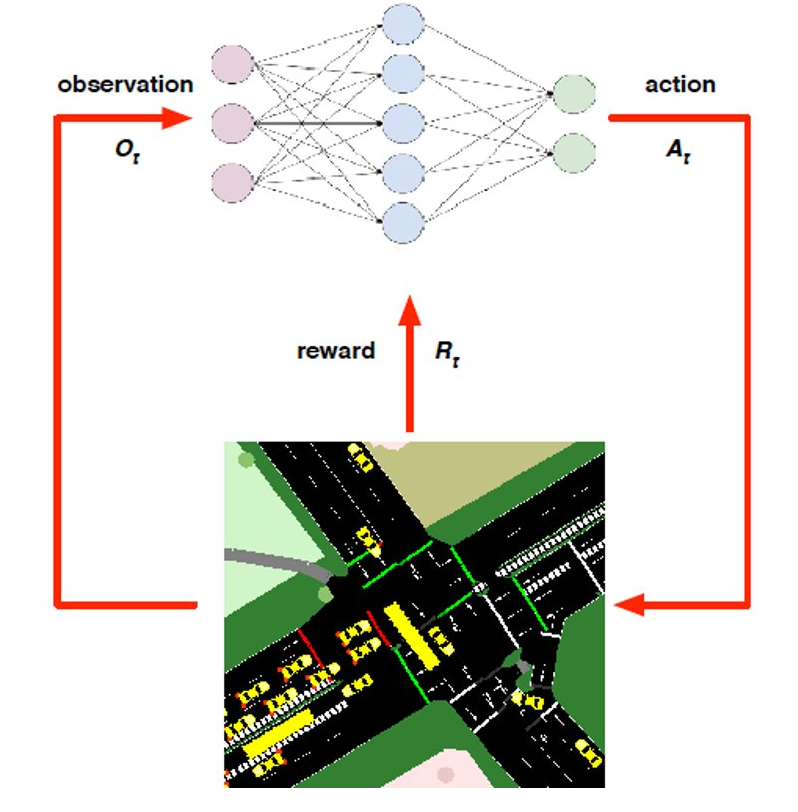
\includegraphics[width=2.5in]{rl}                                    
\caption{Study Junction model in SUMO}                                  
\label{rl}                                               
\end{figure}     

\subsection{Reinforcement Learning Agent}

\subsection{Reinforcement Learning Environment}

\begin{figure}                                                
\centering                                                    
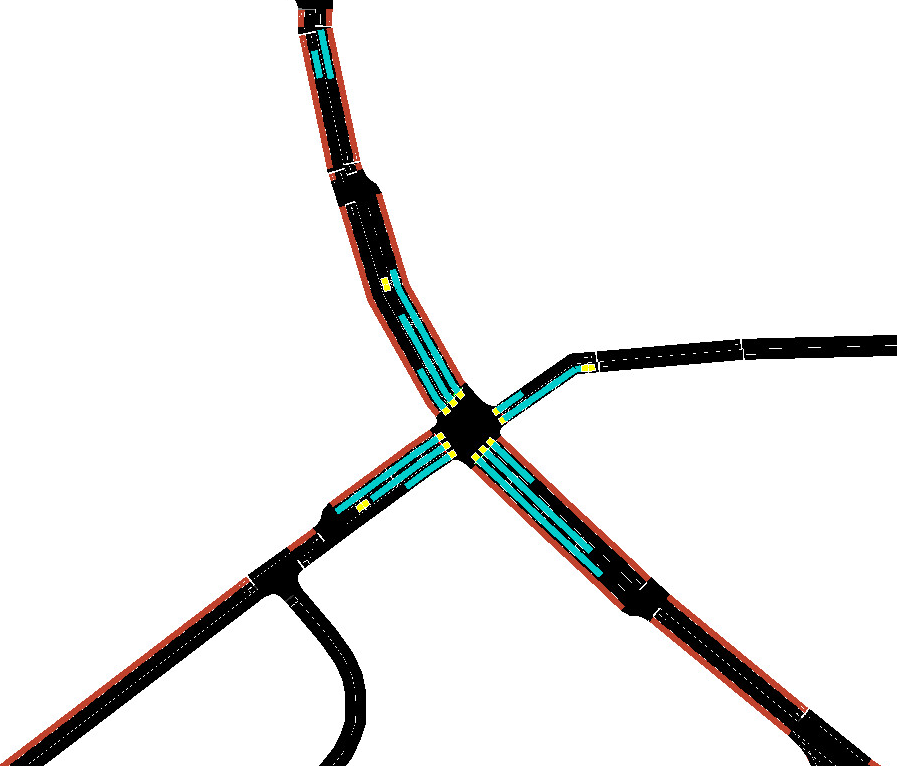
\includegraphics[width=2.5in]{intersection}                                    
\caption{Study Junction model in SUMO}                                  
\label{intersection}                                               
\end{figure}     

\subsection{State Representation}

\subsection{Actions of the Agent}


\section{Reward Functions}

\subsection{Queue based Reward Functions}

\subsection{Waiting Time based Rewards Functions}

\subsection{Delay Based Reward Functions}

\subsection{Average Speed Reward Functions}


\section{Experiments}

\subsection{Training Process}

\subsection{Evaluation and Scoring}


\section{Results}

\section{Discussion and Conclusion}



% Reminder: the "draftcls" or "draftclsnofoot", not "draft", class option
% should be used if it is desired that the figures are to be displayed while
% in draft mode.

% An example of a floating figure using the graphicx package.
% Note that \label must occur AFTER (or within) \caption.
% For figures, \caption should occur after the \includegraphics.
%
%\begin{figure}
%\centering
%\includegraphics[width=2.5in]{myfigure}
% where an .eps filename suffix will be assumed under latex, 
% and a .pdf suffix will be assumed for pdflatex
%\caption{Simulation Results}
%\label{fig_sim}
%\end{figure}


% An example of a double column floating figure using two subfigures.
%(The subfigure.sty package must be loaded for this to work.)
% The subfigure \label commands are set within each subfigure command, the
% \label for the overall fgure must come after \caption.
% \hfil must be used as a separator to get equal spacing
%
%\begin{figure*}
%\centerline{\subfigure[Case I]{\includegraphics[width=2.5in]{subfigcase1}
% where an .eps filename suffix will be assumed under latex, 
% and a .pdf suffix will be assumed for pdflatex
%\label{fig_first_case}}
%\hfil
%\subfigure[Case II]{\includegraphics[width=2.5in]{subfigcase2}
% where an .eps filename suffix will be assumed under latex, 
% and a .pdf suffix will be assumed for pdflatex
%\label{fig_second_case}}}
%\caption{Simulation results}
%\label{fig_sim}
%\end{figure*}



% An example of a floating table. Note that, for IEEE style tables, the 
% \caption command should come BEFORE the table. Table text will default to
% \footnotesize as IEEE normally uses this smaller font for tables.
% The \label must come after \caption as always.
%
%\begin{table}
%% increase table row spacing, adjust to taste
%\renewcommand{\arraystretch}{1.3}
%\caption{An Example of a Table}
%\label{table_example}
%\begin{center}
%% Some packages, such as MDW tools, offer better commands for making tables
%% than the plain LaTeX2e tabular which is used here.
%\begin{tabular}{|c||c|}
%\hline
%One & Two\\
%\hline
%Three & Four\\
%\hline
%\end{tabular}
%\end{center}
%\end{table}




% conference papers do not normally have an appendix

% use section* for acknowledgement
\section*{Acknowledgment}
% optional entry into table of contents (if used)
%\addcontentsline{toc}{section}{Acknowledgment}
This work was part funded by InnovateUK grant 104219 andpart funded by EPSRC Grant EP/L015374. 
We are also grateful to W. Chernikoff, Toyota Mobility Foundation and The Alan Turing Institute for support in the initial stages.






% trigger a \newpage just before the given reference
% number - used to balance the columns on the last page
% adjust value as needed - may need to be readjusted if
% the document is modified later
%\IEEEtriggeratref{8}
% The "triggered" command can be changed if desired:
%\IEEEtriggercmd{\enlargethispage{-5in}}

% references section
% NOTE: BibTeX documentation can be easily obtained at:
% http://www.ctan.org/tex-archive/biblio/bibtex/contrib/doc/

% can use a bibliography generated by BibTeX as a .bbl file
% standard IEEE bibliography style from:
% http://www.ctan.org/tex-archive/macros/latex/contrib/supported/IEEEtran/bibtex
%\bibliographystyle{IEEEtran.bst}
% argument is your BibTeX string definitions and bibliography database(s)
%\bibliography{IEEEabrv,../bib/paper}
%
% <OR> manually copy in the resultant .bbl file
% set second argument of \begin to the number of references
% (used to reserve space for the reference number labels box)
\begin{thebibliography}{1}

\bibitem{IEEEhowto:kopka}
H.~Kopka and P.~W. Daly, \emph{A Guide to {\LaTeX}}, 3rd~ed.\hskip 1em plus
  0.5em minus 0.4em\relax Harlow, England: Addison-Wesley, 1999.

\end{thebibliography}


% that's all folks
\end{document}


